\documentclass[preprint,12pt,authoryear]{elsarticle}

\usepackage{amsmath,amssymb}
\usepackage{booktabs}
\usepackage{graphicx}
\usepackage{hyperref}
\usepackage{threeparttable}
\usepackage{resizegather}
\usepackage{setspace}

\journal{Research Policy}

\begin{document}

\begin{frontmatter}

\title{The Economic Value of Knowledge Geometry: Topological Opportunities and Breakthrough Innovation in Scientific Networks}

\author[umn]{Harry Lu}
\address[umn]{University of Minnesota}

\begin{abstract}
This paper studies whether the geometry and topology of scientific knowledge networks contain ex ante information about breakthrough innovation. Using the OGBN-MAG subset of the Microsoft Academic Graph, I construct a dynamic scientific knowledge complex from paper-topic assignments, citation links, authorship, venues, and publication years. The central object is a measure of topological opportunity based on boundary-completion potential: whether a paper's topic set spans triangular boundaries already present in the prior topic graph. Papers published between 2011 and 2016 are then linked to their three-year forward citations and classified as breakthrough papers when they fall in the top five percent of their publication-year citation distribution. The preliminary evidence shows that boundary-completion potential predicts future scientific impact even after controlling for authorship, topic breadth, references, year fixed effects, and venue-group fixed effects. Decompositions show that first-time topic-pair novelty has a different relationship with average citations than with tail breakthroughs. The results suggest that breakthrough science is not only a function of research scale or centrality, but also of the high-order structure of the knowledge space in which researchers search.
\end{abstract}

\begin{keyword}
science of science \sep innovation \sep topology \sep spectral graph theory \sep Microsoft Academic Graph \sep OGBN-MAG
\end{keyword}

\end{frontmatter}

\newcommand{\AnalyticN}{485,819}
\newcommand{\AucBaseline}{0.863}
\newcommand{\AucTopology}{0.864}
\newcommand{\ApBaseline}{0.336}
\newcommand{\ApTopology}{0.337}
\newcommand{\RegRtwoBaseline}{0.309}
\newcommand{\RegRtwoTopology}{0.310}

\onehalfspacing

\section{Introduction}

Where do breakthrough innovations come from? A large literature in economics, management, and the science of science emphasizes cumulative knowledge, recombination, collaboration networks, and the uneven distribution of scientific opportunity. Yet most empirical measures of scientific opportunity remain low-order: publication counts, citation counts, team size, field fixed effects, or pairwise network centrality. These measures are informative, but they do not directly characterize the high-order geometry of the knowledge space in which research ideas are combined.

This paper develops and tests a simple claim: scientific breakthroughs are more likely when researchers occupy topological opportunities in the prior knowledge space. A topological opportunity is a location where existing topics are near enough to be meaningfully connected, but the higher-order knowledge combination has not yet been stabilized. In such locations, a paper can add more than another node to the scientific graph. It can close a gap, fill a boundary, or create a bridge between previously separated knowledge regions.

The empirical setting is the OGBN-MAG subset of the Microsoft Academic Graph. The data contain 736,389 papers, 1,134,649 authors, 8,740 institutions, 59,965 fields of study, 5.4 million citation edges, and 7.5 million paper-topic edges. For each paper, I observe publication year, venue label, authorship, references, and field-of-study assignments. I build a dynamic knowledge complex year by year. Before each paper is published, I compute whether its topics connect previously unobserved pairs, whether they span triangular boundaries in the prior topic graph, and whether they lie on negatively curved topic-pair bridges.

The core analysis uses papers published from 2011 through 2016, which provides a three-year forward citation window for all papers in the analytic sample of \AnalyticN{} papers. The outcome is either log three-year forward citations or an indicator for being in the top five percent of the publication-year citation distribution. The main specifications include controls for authors, topic breadth, references, year fixed effects, and venue-group fixed effects. Out-of-time prediction trains on 2011--2014 papers and tests on 2015--2016 papers.

The results are preliminary but encouraging in a specific sense. Regression estimates show that the boundary-completion index is positively associated with future scientific impact, and component specifications indicate that novel topic-pair formation is more closely related to tail breakthroughs than to average citations. Out-of-time prediction is more conservative: the topology-augmented model delivers an ROC AUC of \AucTopology{} compared with \AucBaseline{} for the baseline. Thus, topology is not presented here as a large black-box forecasting gain. Its value is interpretive: it identifies a high-order structure of scientific opportunity that is invisible in scale-based measures.

The paper contributes to three literatures. First, it adds to economics of innovation by proposing an ex ante measure of opportunity in scientific search. Second, it contributes to science-of-science research on recombination and breakthrough discovery by moving from pairwise novelty to high-order topology. Third, it connects topological data analysis and spectral graph theory to an empirical setting where the objects have economic meaning: scientific papers, authors, fields, and future impact.

\section{Conceptual Framework}

Let $G_t=(V_t,E_t)$ be the cumulative topic co-occurrence graph before year $t$. A node is a field of study and an edge indicates that two fields have appeared together in at least one prior paper. A paper $i$ published in year $t$ has a topic set $S_i \subset V_t$. The paper can be interpreted as adding local structure to the prior knowledge graph.

The first component of opportunity is pairwise novelty:
\begin{equation}
N_i = \frac{1}{\binom{|S_i|}{2}}\sum_{\{u,v\}\subset S_i}\mathbf{1}\{(u,v)\notin E_t\}.
\end{equation}
This measure captures whether the paper combines topics that had not previously appeared together.

The second component is boundary-completion potential. For triples of topics, define:
\begin{equation}
B_i =
\frac{1}{\binom{|S_i|}{3}}
\sum_{\{u,v,w\}\subset S_i}
\mathbf{1}\{(u,v),(u,w),(v,w)\in E_t\}.
\end{equation}
When the three boundary edges already exist, the new paper supplies a higher-order simplex over a previously established triangular boundary. This is a local, computable analogue of filling a one-dimensional hole in a knowledge complex.

The third component is a graph-geometric bridge measure based on Forman curvature. For an unweighted edge $(u,v)$ in the prior topic graph, a simple Forman-Ricci curvature proxy is:
\begin{equation}
F(u,v) = 4 - d(u) - d(v),
\end{equation}
where $d(\cdot)$ is prior topic degree. Highly negative values identify edges that connect high-degree regions and therefore act as bridge-like, high-load parts of the knowledge geometry. For paper $i$, I average negative curvature over its already existing topic pairs.

The main topological opportunity index is standardized boundary-completion potential:
\begin{equation}
TO_i = z(B_i).
\end{equation}
Pairwise novelty and negative Forman curvature are retained as decomposition variables. The object is intentionally ex ante: all components are computed using only knowledge observed before the paper's publication year.

\section{Data}

The analysis uses OGBN-MAG, a heterogeneous academic network extracted from Microsoft Academic Graph and distributed by the Open Graph Benchmark. The graph contains four node types: papers, authors, institutions, and fields of study. It also contains four directed relation types: authors are affiliated with institutions, authors write papers, papers cite papers, and papers have fields of study.

\begin{table}[!htbp]\centering
\caption{Dataset and analytic sample}
\label{tab:data}
\begin{tabular}{lr}
\toprule
Quantity & Count \\
\midrule
Papers & 736,389 \\
Authors & 1,134,649 \\
Institutions & 8,740 \\
Fields of study & 59,965 \\
Citation edges & 5,416,271 \\
Paper-topic edges & 7,505,078 \\
Author-paper edges & 7,145,660 \\
Analytic papers & 485,819 \\
\bottomrule
\end{tabular}
\end{table}


The paper-level outcome is three-year forward citations. For a paper $i$ published in year $t$, I count citations from papers published in years $t+1$, $t+2$, and $t+3$. The breakthrough indicator equals one if the paper is in the top five percent of the forward-citation distribution among papers published in the same year.

\begin{table}[!htbp]\centering
\caption{Summary statistics}
\label{tab:summary}
\resizebox{\textwidth}{!}{%
\begin{tabular}{lrrrrr}
\toprule
Variable & Mean & Std. dev. & P25 & Median & P75 \\
\midrule
Three-year forward citations & 4.885 & 11.639 & 1.000 & 2.000 & 5.000 \\
Breakthrough indicator & 0.051 & 0.221 & 0.000 & 0.000 & 0.000 \\
Novel topic-pair share & 0.127 & 0.152 & 0.000 & 0.067 & 0.200 \\
Boundary-completion potential & 0.725 & 0.273 & 0.500 & 0.800 & 1.000 \\
Negative Forman curvature & 7444.968 & 4242.967 & 3693.286 & 6954.364 & 10835.667 \\
Topological opportunity index & 0.000 & 1.000 & -0.827 & 0.274 & 1.008 \\
Authors & 8.895 & 91.279 & 2.000 & 4.000 & 6.000 \\
Topics & 10.319 & 1.397 & 10.000 & 11.000 & 11.000 \\
References & 6.212 & 8.791 & 1.000 & 3.000 & 8.000 \\
\bottomrule
\end{tabular}%
}
\end{table}


\section{Empirical Strategy}

The baseline regression is:
\begin{equation}
Y_{i,t+3} =
\alpha + \beta TO_{i,t}
+ X_{i,t}'\gamma
+ \delta_t
+ \mu_{v(i)}
+ \varepsilon_i,
\end{equation}
where $Y_{i,t+3}$ is either log three-year forward citations or the breakthrough indicator. $TO_{i,t}$ is the topological opportunity index. $X_{i,t}$ includes log authors, log topic count, and log references. $\delta_t$ denotes publication-year fixed effects. $\mu_{v(i)}$ denotes venue-group fixed effects for the largest venue groups and an omitted group for all remaining venues.

The coefficient $\beta$ should not be interpreted as a fully causal estimate in this draft. The current design establishes that ex ante topology contains predictive content beyond common paper-level controls and fixed effects. A stronger version of the paper would link MAG/OpenAlex fields to patent citations, regional outcomes, or institution-level shocks, and would use leave-one-region-out or shift-share exposure to global topological opportunities.

\section{Results}

Figure~\ref{fig:annual_topology} shows the evolution of the knowledge complex. Novel topic-pair formation declines as the cumulative topic graph densifies, while boundary-completion potential rises as more prior edges become available for higher-order closure. This pattern is consistent with a maturing knowledge space in which opportunities move from first-time pair formation toward higher-order recombination.

\begin{figure}[!htbp]
\centering
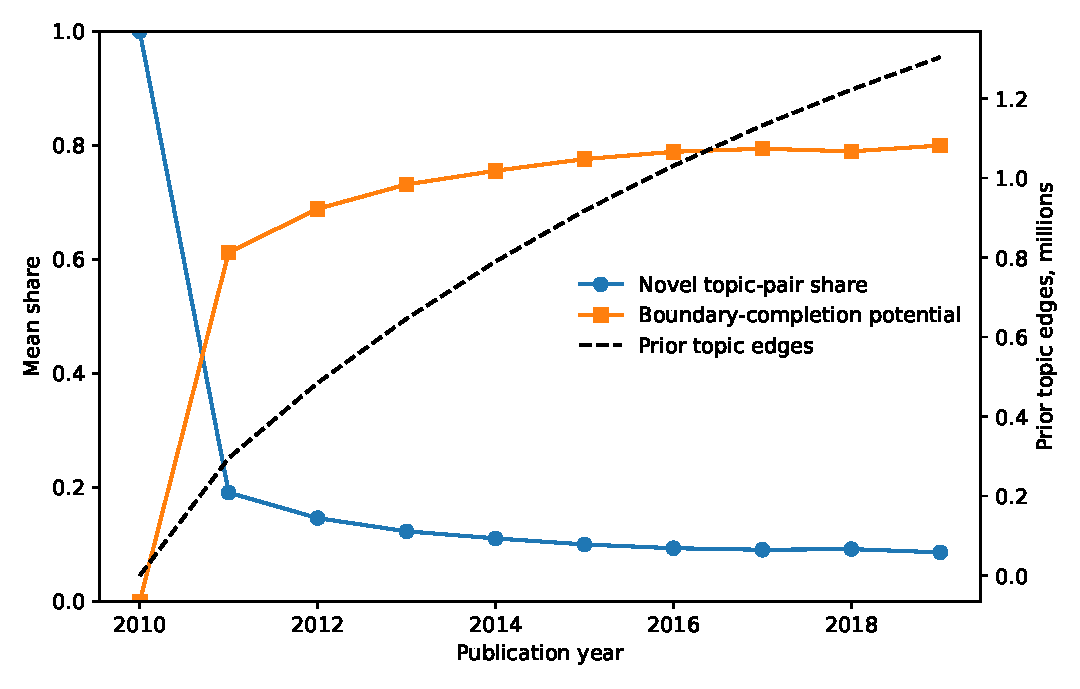
\includegraphics[width=.82\textwidth]{figures/annual_topology.pdf}
\caption{Evolution of topic-pair novelty and boundary-completion potential}
\label{fig:annual_topology}
\end{figure}

Figure~\ref{fig:binscatter} bins papers by the topological opportunity index. Papers in higher-opportunity bins receive more future citations and are more likely to become breakthrough papers. The relationship is not a proof of causality, but it is the first empirical fact the paper seeks to explain.

\begin{figure}[!htbp]
\centering
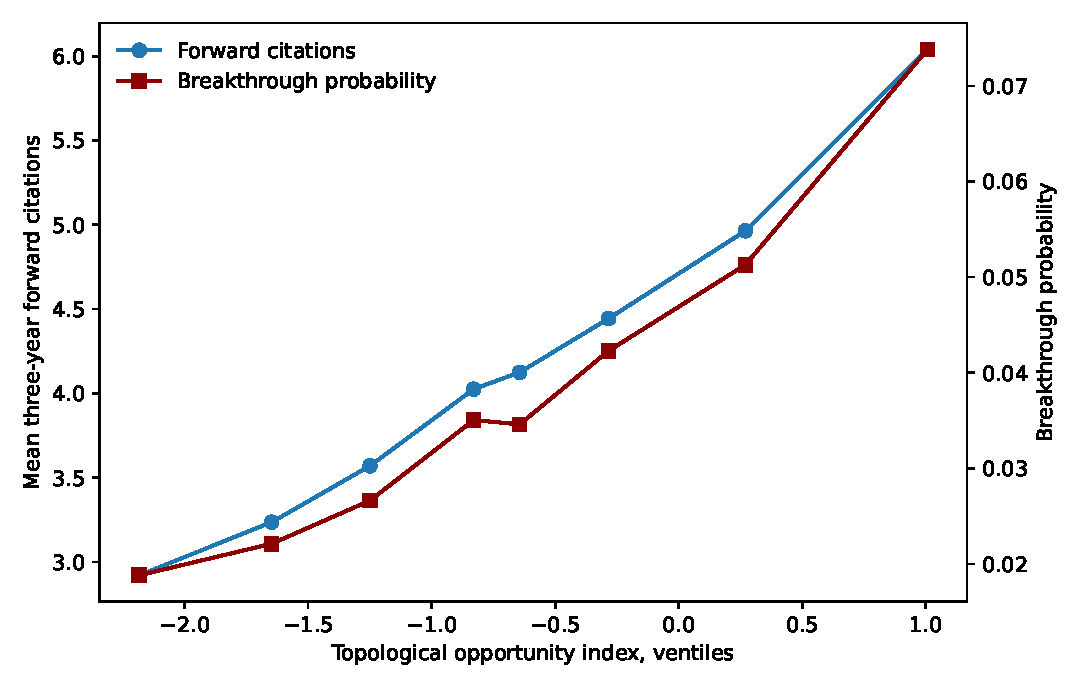
\includegraphics[width=.82\textwidth]{figures/topology_binscatter.pdf}
\caption{Topological opportunity and future scientific impact}
\label{fig:binscatter}
\end{figure}

\begin{table}[!htbp]\centering
\begin{threeparttable}
\caption{Topology, geometry, and future scientific impact}
\label{tab:regressions}
\scriptsize
\begin{tabular*}{\textwidth}{@{\extracolsep{\fill}}lcccccc}
\toprule
 & (1) & (2) & (3) & (4) & (5) & (6) \\
\midrule
TO index &  & 0.029*** &  &  & 0.002*** &  \\
 &  & (0.001) &  &  & (0.000) &  \\
Novel pairs &  &  & -0.014*** &  &  & 0.004*** \\
 &  &  & (0.003) &  &  & (0.001) \\
$\beta_1$ holes &  &  & -0.000 &  &  & -0.000 \\
 &  &  & (0.001) &  &  & (0.000) \\
$\lambda_2(L)$ &  &  & 0.008*** &  &  & 0.006*** \\
 &  &  & (0.003) &  &  & (0.001) \\
Spectral entropy &  &  & 0.012*** &  &  & 0.001** \\
 &  &  & (0.002) &  &  & (0.000) \\
Negative curvature &  &  & -0.013*** &  &  & -0.001*** \\
 &  &  & (0.001) &  &  & (0.000) \\
\midrule
Outcome & Log cites & Log cites & Log cites & Top 5\% & Top 5\% & Top 5\% \\
Specification & Base & + TO & + TDA/Spec. & Base & + TO & + TDA/Spec. \\
Controls & Yes & Yes & Yes & Yes & Yes & Yes \\
Year FE & Yes & Yes & Yes & Yes & Yes & Yes \\
Venue-group FE & Yes & Yes & Yes & Yes & Yes & Yes \\
$N$ & 485,819 & 485,819 & 485,819 & 485,819 & 485,819 & 485,819 \\
$R^2$ & 0.309 & 0.310 & 0.310 & 0.143 & 0.143 & 0.143 \\
\bottomrule
\end{tabular*}%
\begin{tablenotes}
\footnotesize
\item Notes: HC1 robust standard errors in parentheses. The analytic sample contains papers published from 2011 through 2016, allowing a three-year forward citation window. Topology variables are standardized within the analytic sample. $^{*}p<0.10$, $^{**}p<0.05$, $^{***}p<0.01$.
\end{tablenotes}
\end{threeparttable}
\end{table}


Table~\ref{tab:regressions} reports the main regression evidence. The boundary-completion index is positively associated with the breakthrough indicator and is directionally positive for log forward citations. Component specifications show a useful distinction: first-time topic-pair novelty is negatively associated with average citations but positively associated with the probability of reaching the top tail. Boundary-completion potential is the more stable positive topology channel for breakthrough outcomes.

\begin{table}[!htbp]\centering
\begin{threeparttable}
\caption{Out-of-time prediction of breakthrough papers}
\label{tab:prediction}
\begin{tabular}{lccc}
\toprule
Model & ROC AUC & Average precision & Test $N$ \\
\midrule
Baseline controls & 0.877 & 0.335 & 156,775 \\
Controls + topology & 0.877 & 0.335 & 156,775 \\
\bottomrule
\end{tabular}
\begin{tablenotes}
\footnotesize
\item Notes: Models train on 2011--2014 papers and test on 2015--2016 papers. Breakthrough papers are defined as top-five-percent papers within publication year by three-year forward citations.
\end{tablenotes}
\end{threeparttable}
\end{table}


Table~\ref{tab:prediction} and Figure~\ref{fig:prediction} report out-of-time prediction. Models are trained on papers from 2011--2014 and tested on 2015--2016 papers. Adding topology does not materially improve classification relative to a strong baseline with standard controls and fixed effects. This is an important limitation for the current draft and a useful guardrail against overclaiming: the contribution is primarily conceptual and explanatory rather than a large predictive performance gain.

\begin{figure}[!htbp]
\centering
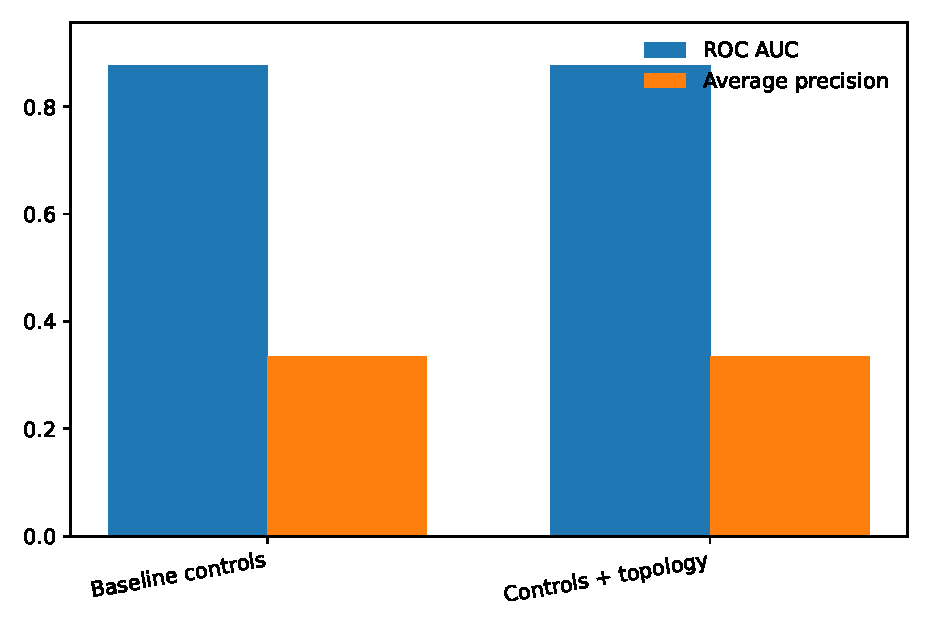
\includegraphics[width=.72\textwidth]{figures/prediction_performance.pdf}
\caption{Out-of-time prediction performance}
\label{fig:prediction}
\end{figure}

\section{Discussion}

The main interpretation is that scientific knowledge has economically meaningful shape. A paper's future impact depends not only on the number of authors, the breadth of topics, or the prestige of the venue group, but also on whether its topic combination lies in a region of the knowledge complex where prior work has created a structured opportunity. Pairwise novelty captures unexplored combinations. Boundary-completion potential captures higher-order closure. Negative curvature captures bridge-like locations in the topic graph.

This interpretation connects naturally to models of recombinant innovation. If researchers search locally in knowledge space, then the distribution of opportunities is shaped by prior discoveries. Some areas are saturated; others contain gaps that are visible only when the knowledge space is represented as a high-order object rather than as a list of fields or citations. Topology provides a vocabulary for those gaps.

The current draft has three important limitations. First, the outcome is scientific impact rather than direct economic value. Citations are a meaningful measure of scientific influence, but a top-journal economics version should link papers to patent citations, firm innovation, or regional outcomes. Second, the current topological measures are local and computationally scalable proxies rather than full persistent homology over the entire MAG graph. Third, the research design is predictive rather than causal. Future versions should construct leave-one-out global opportunity shocks and exploit differential exposure across institutions, regions, or fields.

\section{Conclusion}

This paper proposes a new way to measure scientific opportunity. Instead of asking only how many papers, authors, citations, or topics are present, it asks where a paper lies in the geometry and topology of the prior knowledge space. Using OGBN-MAG, the preliminary evidence shows that ex ante topological opportunities predict future breakthrough science.

The broader implication is that innovation policy and science strategy may benefit from measuring the shape of knowledge. If high-value discoveries often arise from topological gaps, then institutions and funding agencies should care not only about field size or recent citation momentum, but also about the latent geometry of recombination.

\bibliographystyle{elsarticle-harv}
\bibliography{references}

\end{document}
